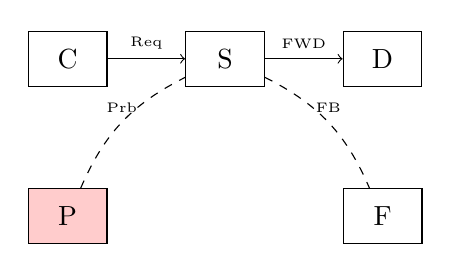
\begin{tikzpicture}[
    scale=0.4,
    node distance=2cm,
    censor/.style={rectangle,draw,fill=red!20,minimum width=1cm,minimum height=0.7cm},
    proxy/.style={rectangle,draw,minimum width=1cm,minimum height=0.7cm},
    client/.style={rectangle,draw,minimum width=1cm,minimum height=0.7cm},
    destination/.style={rectangle,draw,minimum width=1cm,minimum height=0.7cm},
    webserver/.style={rectangle,draw,minimum width=1cm,minimum height=0.7cm}
]

    \node[client] (client) {C};
    \node[censor] (censor) [below of=client] {P};
    \node[proxy] (proxy) [right of=client] {S};
    \node[destination] (destination) [right of=proxy] {D};
    \node[webserver] (webserver) [below of=destination] {F};

    \draw[->] (client) to node[above, font=\tiny] {Req} (proxy);
    \draw[dashed] (censor) to[bend left=20] node[above, font=\tiny] {Prb} (proxy);
    \draw[->] (proxy) to node[above, font=\tiny] {FWD} (destination);
    \draw[dashed] (proxy) to[bend left=20] node[above, font=\tiny] {FB} (webserver);
\end{tikzpicture}